\chapter{Methodology}

\section{Overview}

The system is divided into two main components:

\textbf{a) Frontend Development:}

Designed using Figma to prototype user flows and interfaces. The frontend is implemented with ViteJS, chosen for its fast build times and modern developer experience. The application provides two distinct user interfaces:
\begin{itemize}
    \item A \textbf{dashboard for administrators}, supporting management of user accounts, templates, and system settings.
    \item A \textbf{workspace for secretaries and inspectors}, focused on drafting, reviewing, and finalizing accreditation documents.
\end{itemize}

\textbf{b) BackEnd Development:} 

Developed using Node.js, serves as the core processing engine that handles user authentication, manages access permissions, and orchestrates communication between the frontend and the AI module. 

\textbf{c) Database:}

MongoDB is chosen as the primary database due to its flexibility in storing user data, document metadata, and system configurations, which supports the need for scalability and complex querying. Supabase complements this setup by acting as a secure storage solution for uploaded documents and generated reports, ensuring that files remain easily accessible and properly versioned.
\section{AI Integration and Refinement}
\subsection{Overview of PhoGPT}
PhoGPT\cite{phogpt} is a Vietnamese-specific large language model (LLM) developed by VinAI, designed to address the unique linguistic and contextual characteristics of the Vietnamese language. Unlike general-purpose LLMs trained predominantly on English data, PhoGPT is built on top of modern transformer-based architectures and trained on large-scale Vietnamese corpora, including news articles, books, and user-generated content.

This targeted approach enables PhoGPT to understand Vietnamese grammar, idioms, and cultural nuances more effectively than multilingual models. Its capabilities include text summarization, question answering, text generation, and semantic analysis, all adapted to Vietnamese linguistic patterns. As a result, PhoGPT is particularly well-suited for applications that require precise language understanding and generation in Vietnamese, such as educational tools, chatbots, and document analysis systems.

In this project, PhoGPT serves as the core language processing engine. It is further refined to perform specialized tasks like detecting duplicated content, suggesting edits aligned with accreditation criteria, and generating draft sections of reports. By leveraging PhoGPT’s native language strengths, the system aims to deliver higher accuracy and contextual relevance compared to using a generic multilingual LLM.

\section{Requirement Analysis}
The development of an AI-assisted accreditation reporting system begins with a comprehensive requirement analysis to ensure alignment with both functional needs and technical constraints. This analysis considers the unique demands of Vietnamese accreditation processes, the diverse roles of end-users, and the technological capabilities required to support efficient, scalable, and secure operations.

At the core, the system must enable secretaries and inspectors to collaboratively draft, edit, and finalize complex accreditation reports. This requires a user interface that is both intuitive and capable of managing large, structured documents, supporting functionalities such as section-based editing, real-time updates, and role-based access. Administrative users, on the other hand, need a dedicated dashboard to oversee user management, define report templates, monitor project progress, and configure system-wide settings. These requirements inform the choice of a modern, high-performance frontend framework (ViteJS), complemented by detailed UI prototypes created in Figma to visualize user flows and interface interactions.

The backend must handle user authentication, manage document data, and orchestrate integration with AI services, ensuring that all processes remain responsive and secure. Node.js serves this role effectively due to its event-driven architecture and scalability, while MongoDB provides a flexible schema for storing heterogeneous data such as user profiles, document metadata, comments, and review histories. Supabase complements this by securely storing uploaded files, template versions, and generated reports, simplifying file access and version control.

From an AI integration perspective, the system requires a specialized module to enhance document drafting and review processes. This includes parsing bilingual templates, detecting inconsistencies, and suggesting improvements aligned with accreditation standards. To meet this need, the project plans to integrate PhoGPT, refining it for domain-specific tasks such as semantic error detection, content summarization, and language quality checks. This integration must be modular, allowing for updates and improvements without disrupting core system operations.

In addition, the system must support real-time collaboration and maintain detailed audit trails. This ensures transparency and accountability in multi-user environments, especially during high-stakes accreditation periods. Notifications and comment threads must be directly linked to specific sections, forms, or reports to streamline feedback and decision-making. Problems identified during review must be tracked with severity indicators and resolution workflows to maintain compliance and quality.

Security and compliance represent another critical set of requirements. User authentication must be robust, with role-based permissions ensuring that data access aligns with organizational policies. Given the sensitive nature of accreditation data, especially when stored and processed in the cloud, the system must comply with data protection standards and implement encryption for both data at rest and in transit.

Finally, the system must be scalable to support future growth, such as new accreditation templates, additional institutions, and evolving national standards. The choice of technologies—including Node.js, MongoDB, Supabase, and AI integration frameworks—reflects this need for adaptability and long-term maintainability.

\begin{figure}[h]
    \centering
    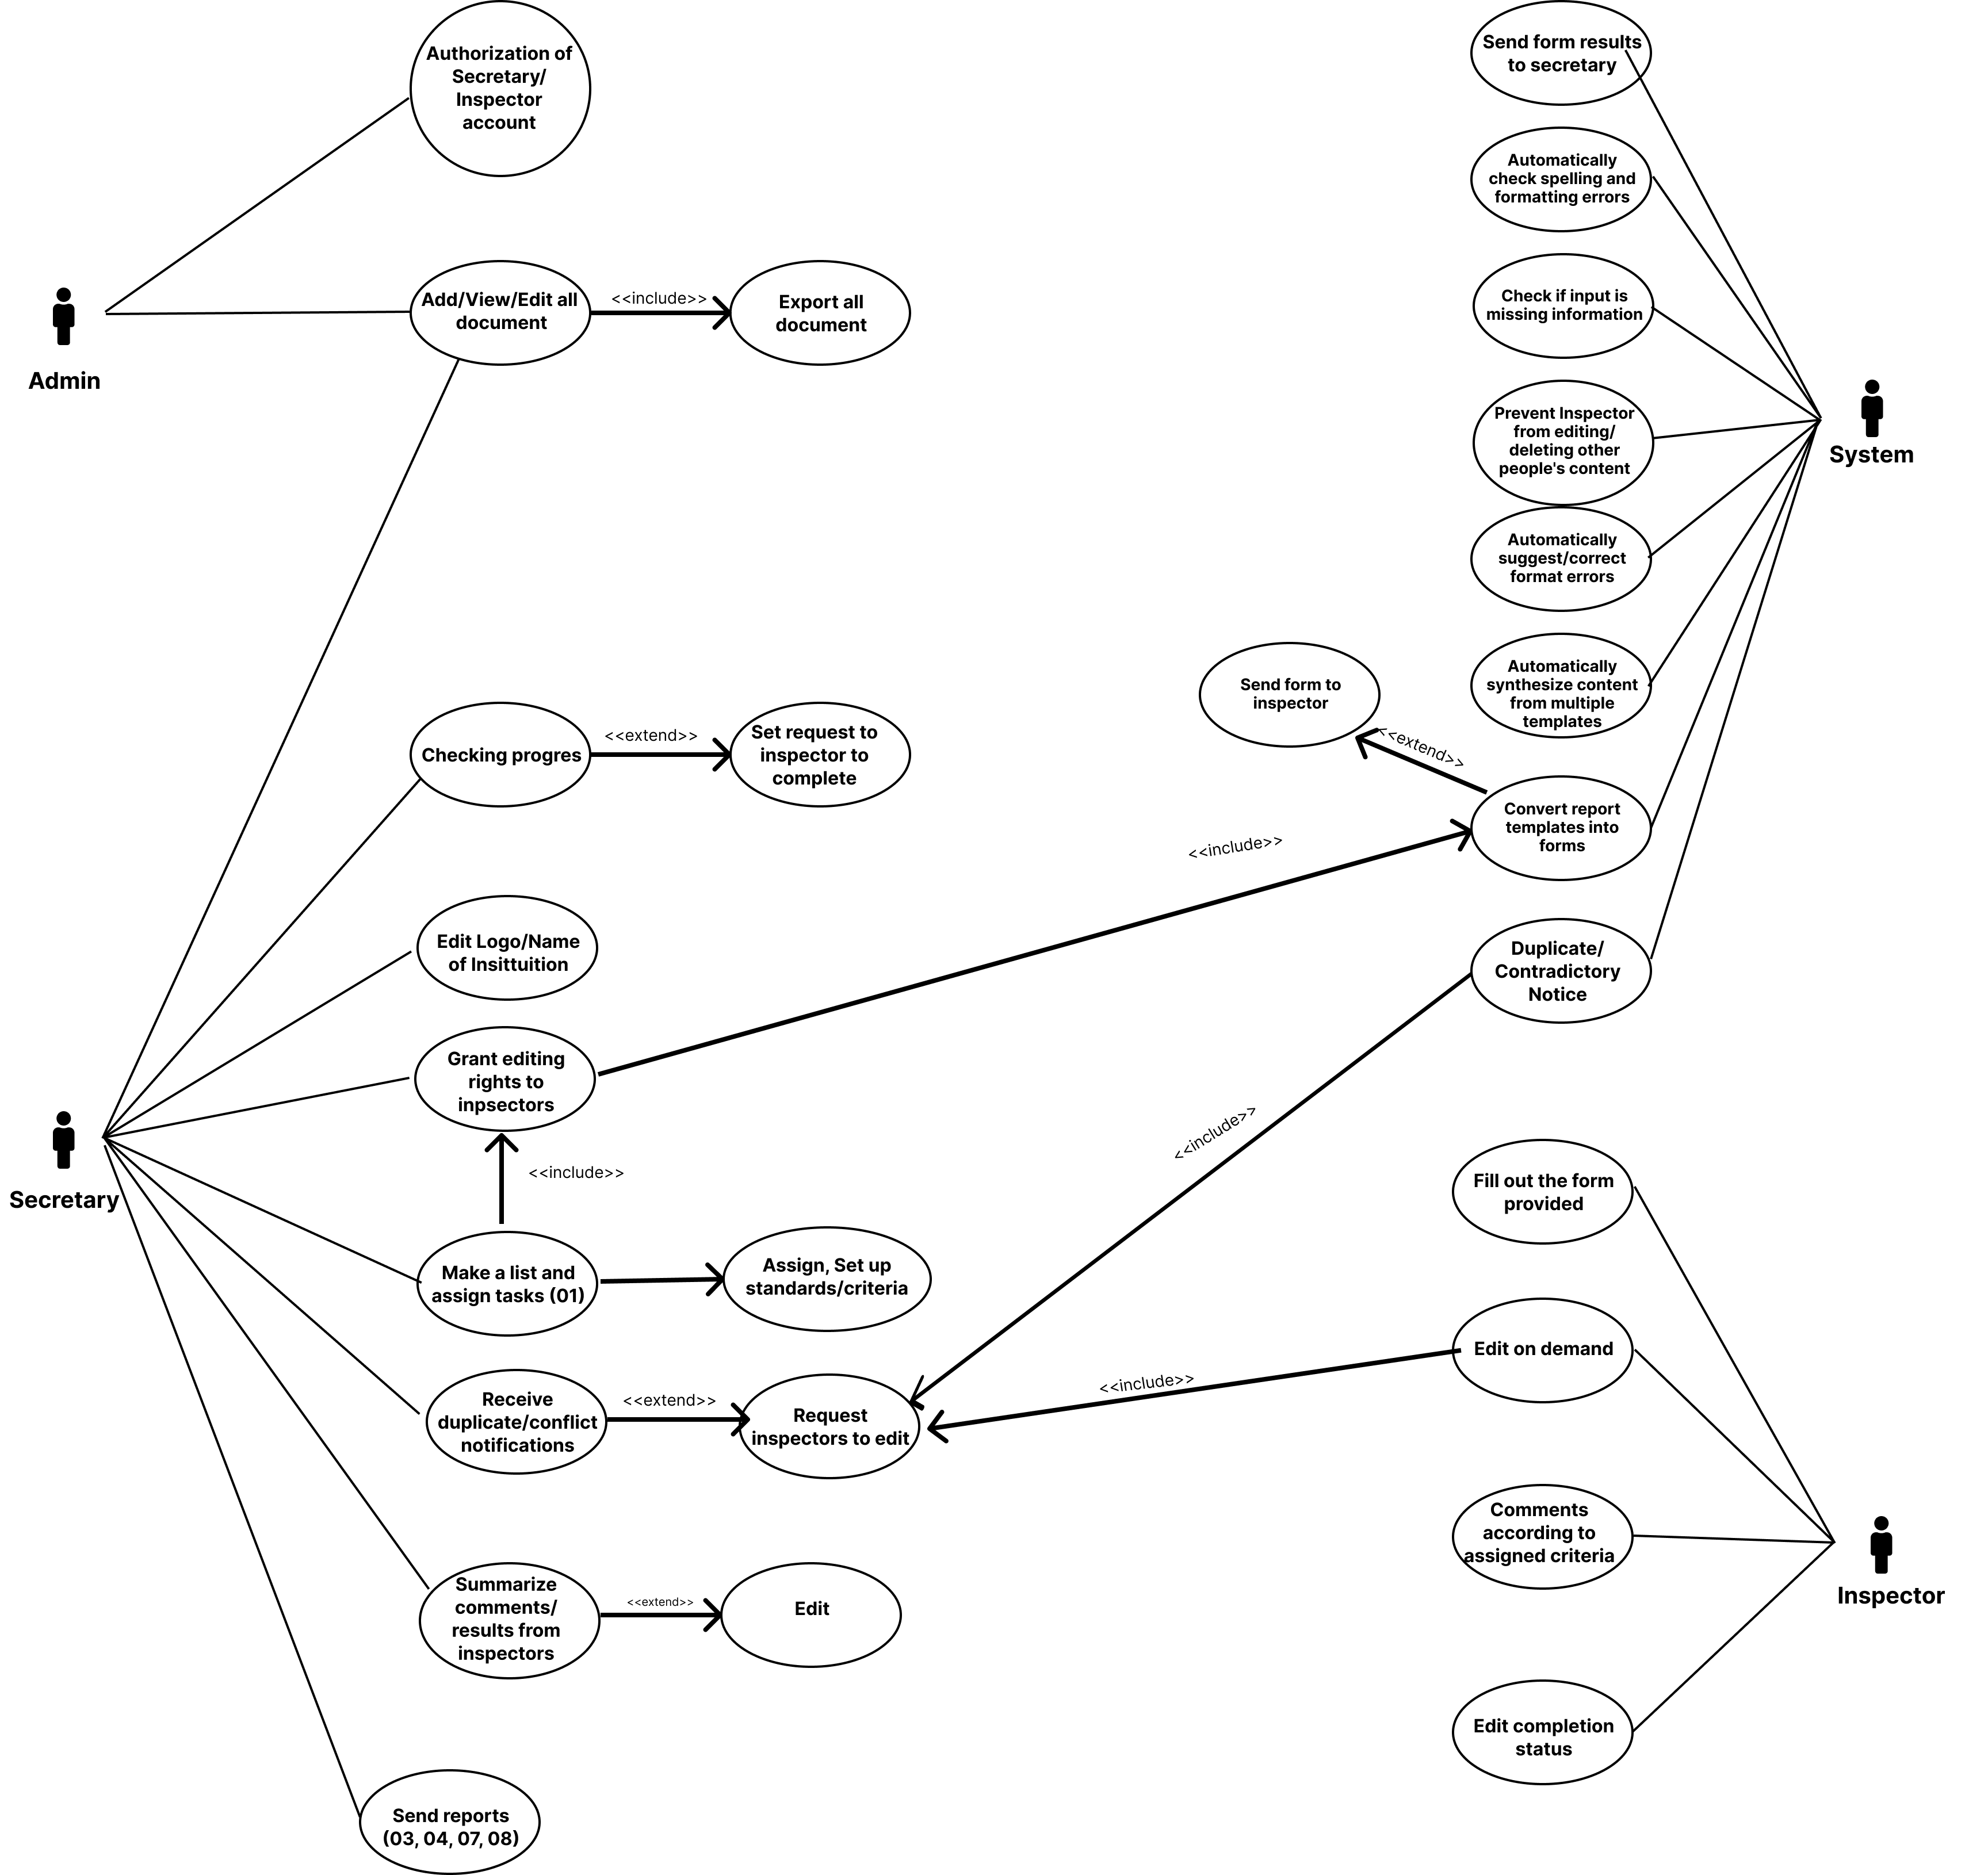
\includegraphics[width=1\textwidth]{images/UCD.png}
    \caption{The Use Case Diagram} 
    \label{fig:usecase}
\end{figure}

Through this requirement analysis, the system is defined not only as a document management tool but as a comprehensive platform that combines workflow automation, AI-enhanced content refinement, and robust collaboration features. This ensures that accreditation teams can focus on substantive content review and quality improvement, supported by a reliable and intelligent digital infrastructure.



\section{Database Design}
To support the complex workflow of accreditation reporting, the system adopts a carefully designed database schema centered on an Evaluation ERD. The design focuses on balancing flexibility, scalability, and clarity, enabling structured collaboration among different user roles and facilitating integration with AI-driven document analysis.

The system’s core entity is Users, which captures essential profile data, authentication information, and user roles such as KĐV, TK, and SuperAdmin. This structure underpins fine-grained access control and workflow assignment across projects and documents. Templates provide reusable blueprints for forms and reports, each linked to its creator and latest editor to ensure accountability and version tracking. Projects serve as containers for coordinated work, storing key metadata like status, completion percentage, deadlines, and assigned members, while explicitly identifying project leaders.

To manage the reporting process, the schema includes Reports tied to specific projects, each with a report type and lifecycle status reflecting its progress from draft to submission. The system also models Forms and their hierarchical structure: each form is associated with a report and can be assigned to specific users for drafting or review. Within forms, Sections divide content into manageable parts, and each section contains Fields where individual pieces of data are entered and tracked for completion.

Supporting collaboration and quality assurance, the ERD integrates several auxiliary entities. Problems capture issues or risks identified during review, linked to the relevant target (project, form, report, field, or section) and tracked by severity and resolution status. Comments allow threaded discussions directly attached to specific content, enabling traceable peer feedback. Reviews formalize evaluation stages for reports, recording reviewer identity, feedback, and approval decisions. Meanwhile, Notifications ensure real-time updates for users by targeting specific entities and indicating urgency levels.

The database schema is relationally linked to maintain data integrity. For instance, reports reference their parent project; forms reference the report and assignee; sections reference the parent form; and fields reference the parent section. 

This ERD not only supports the core workflow—from template-driven report generation to collaborative drafting and final approval—but also prepares the backend to integrate with AI modules such as PhoGPT for content refinement and document analysis. By modeling entities like problems, comments, and reviews explicitly, the system aligns with the accreditation process’s need for traceable edits, iterative feedback, and systematic quality control. Ultimately, this robust and adaptable database design underpins the entire accreditation support system, ensuring scalability and clarity while supporting the domain-specific requirements of Vietnamese accreditation workflows.
\begin{figure}[h]
    \centering
    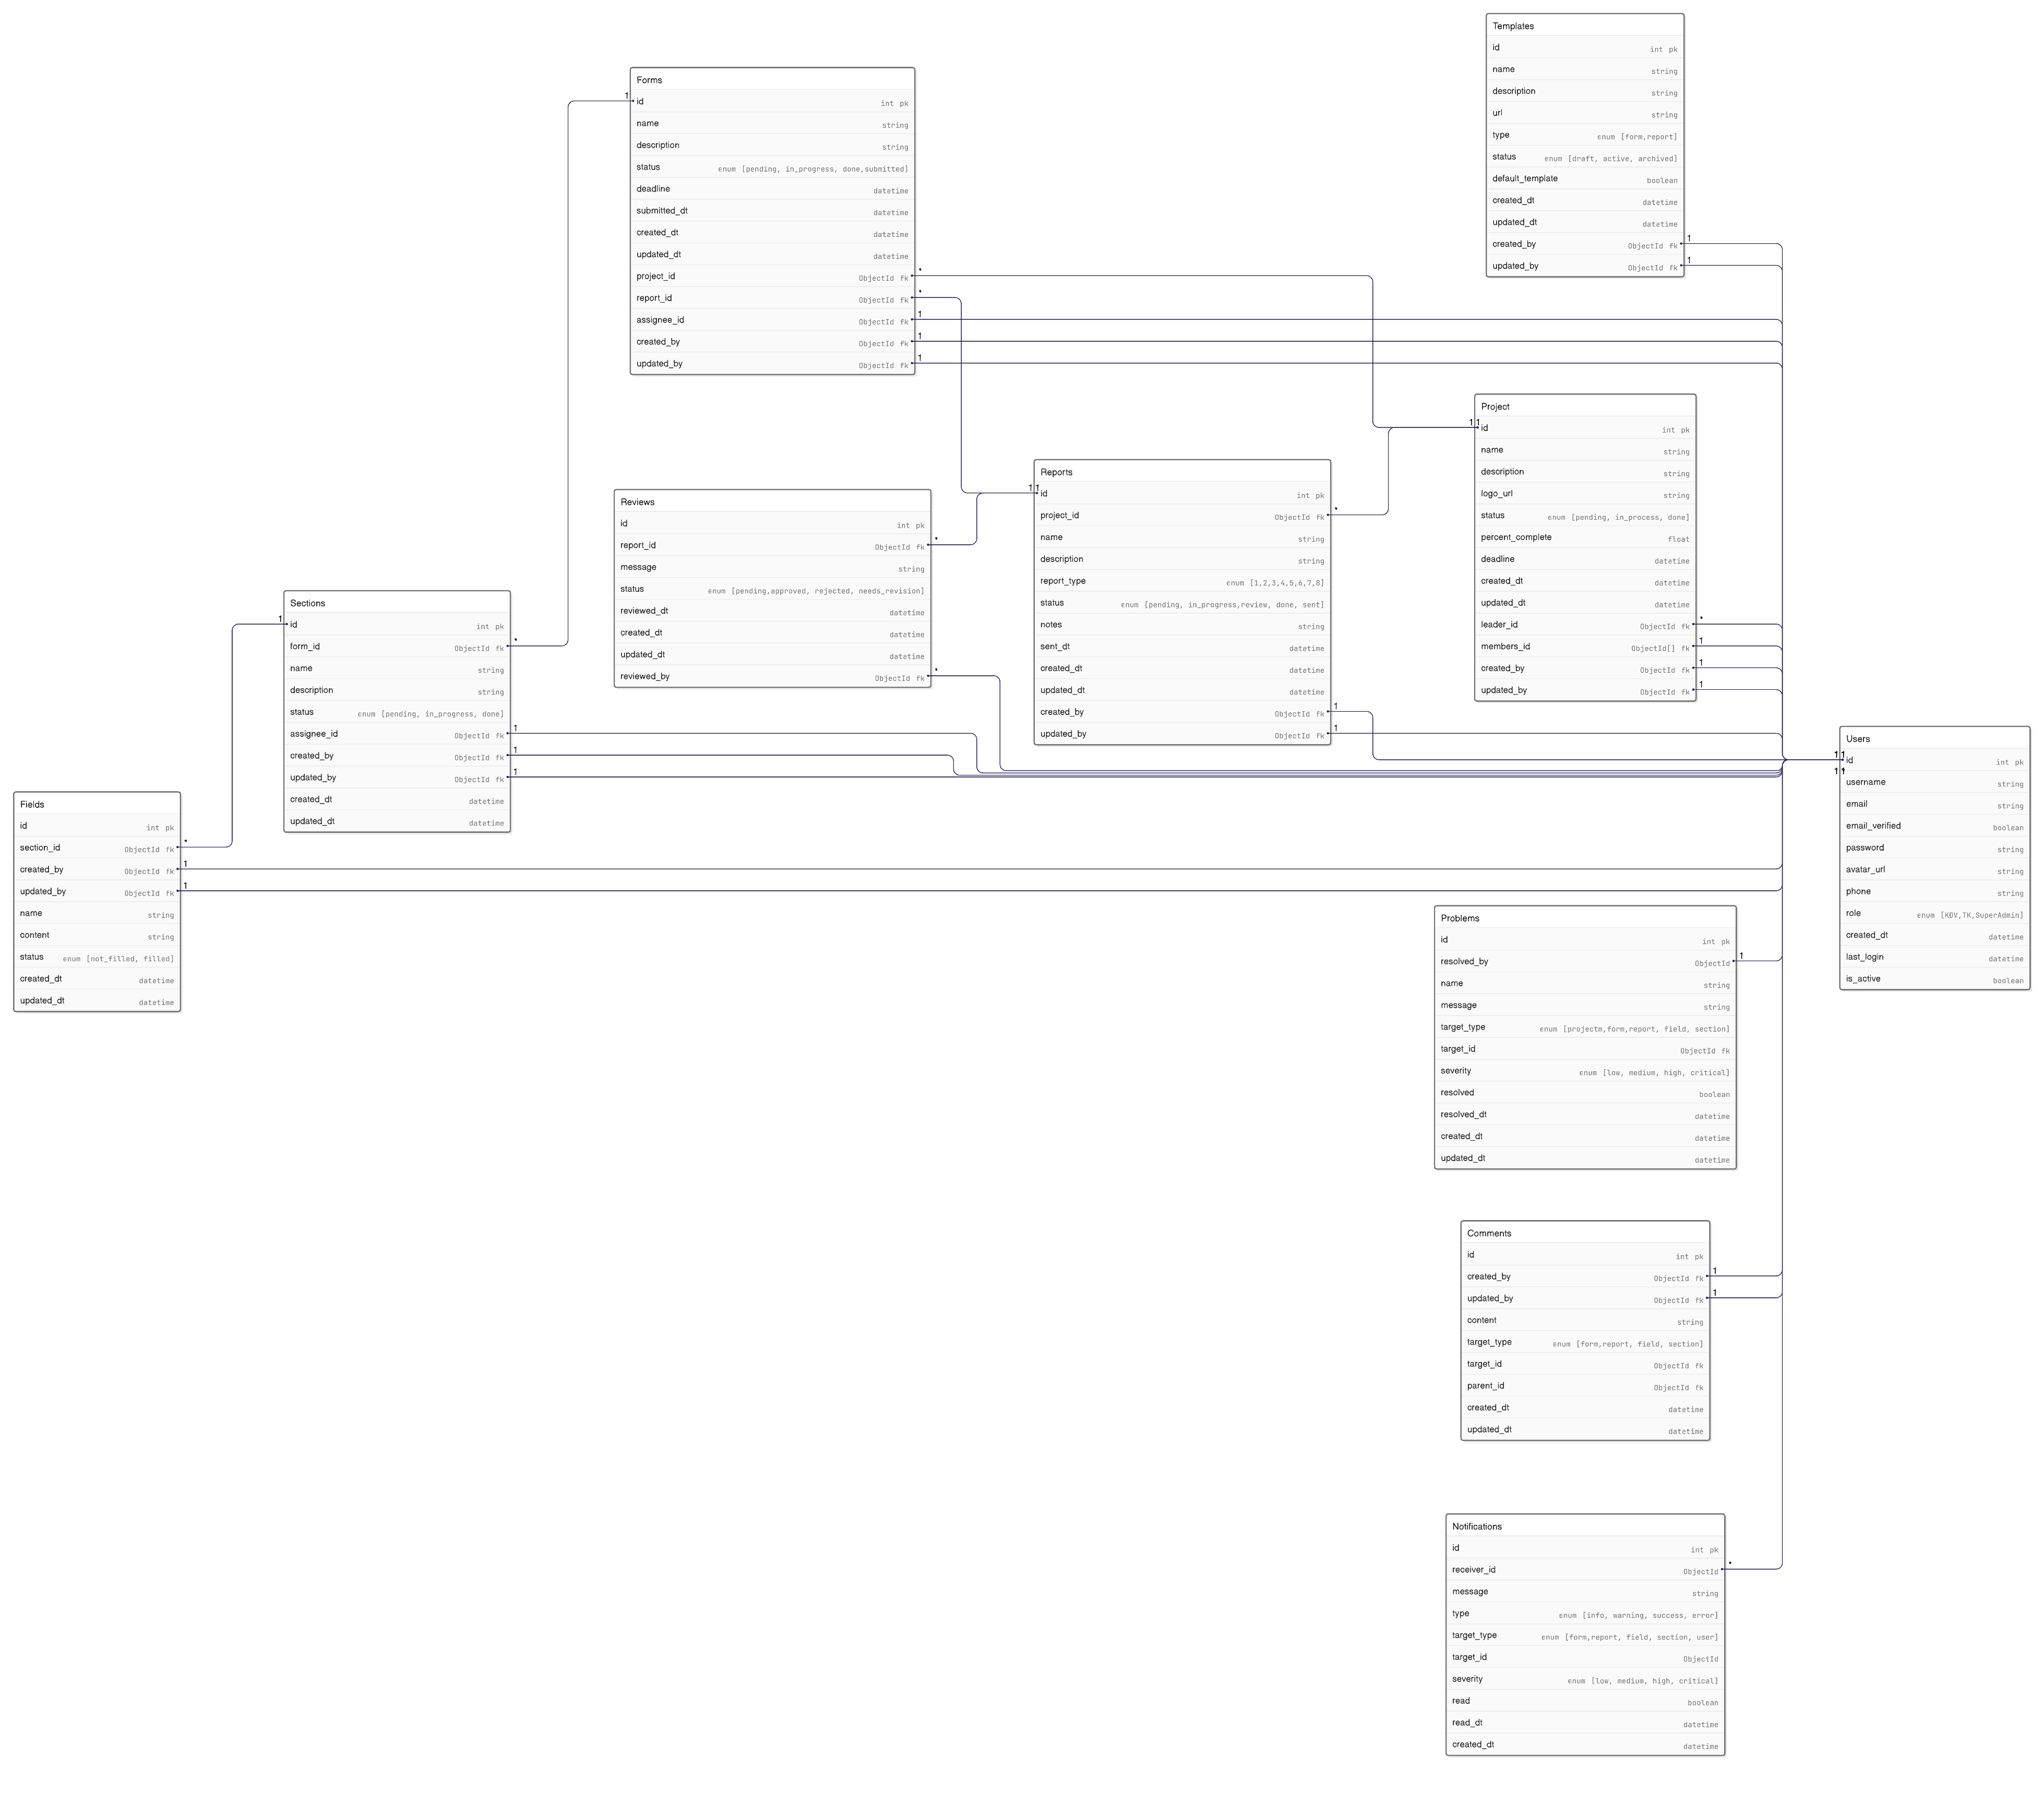
\includegraphics[width=0.5\textwidth]{images/ERD.png}
    \caption{The Entity Relation Diagram} 
    \label{fig:erd}
\end{figure}

\section{AI Integration}

A critical part of the system is the integration of PhoGPT, a large language model pre-trained on Vietnamese data and further refined for the accreditation context. This refinement involves training the model to recognize bilingual document structures, detect duplicated content, identify language errors, and evaluate the completeness and consistency of accreditation reports based on required standards. The AI module operates as a dedicated processing thread in the backend, allowing real-time interaction between users and the AI-powered features. For instance, when a secretary edits a report or uploads a new draft, the backend sends relevant document segments to PhoGPT, which then returns suggestions, content summaries, or error checks. These results are seamlessly displayed in the user interface, guiding users to improve document quality and compliance.
\subsection{Dataset Collection and Preparation}
To build the AI module, a domain-specific dataset was prepared using anonymized accreditation documents provided by institutional archives and authorized departments. This dataset includes past full reports, bilingual (Vietnamese-English) drafts, reviewer comments, and official templates issued by CEA VNU-HCM. Publicly available accreditation guidelines and sample templates were also added to cover structural requirements. Where direct data was unavailable due to confidentiality, synthetic data resembling real accreditation reports was generated to ensure completeness.

Collected documents were preprocessed by normalizing text, removing personal identifiers, and segmenting content into logical units such as sections, fields, and comments. Metadata tags, including language, section type, and related accreditation criteria, were added to support context-aware AI prompting. The final dataset is securely stored in MongoDB for use by the backend during AI-assisted drafting and validation.
\subsection{AI Model Integration and Prompt Engineering}
The project uses PhoGPT, integrated through a dedicated backend thread written in Node.js. When a user requests AI assistance, the backend dynamically generates prompts using project metadata, template context, and user history. These prompts instruct PhoGPT to produce draft text, suggest bilingual edits, or check compliance with accreditation standards.

Instead of full retraining, prompt engineering adapts PhoGPT’s output to match the formal, criteria-driven style required in accreditation. Outputs are post-processed to remove irrelevant content and ensure they align with user roles and project context.

\subsection{Document Drafting and Validation}
The AI supports users by drafting new sections, identifying duplicated content, and suggesting improvements for clarity and compliance. AI-generated drafts and suggestions are stored in Supabase alongside user edits, enabling traceability of what was accepted, revised, or rejected.

To preserve human oversight, the AI only provides recommendations. Secretaries, inspectors, and administrators review, edit, and finalize reports, ensuring responsibility for the final content remains with the users.

\subsection{Security and Ethical Considerations}
Data privacy is maintained by anonymizing documents before they enter the AI workflow. Role-based access control (as designed in the ERD) limits who can view or edit specific data. AI suggestions are advisory, reducing the risk of over-reliance and preserving accountability.